\providecommand{\main}{../../..}
\documentclass[\main/dresen_thesis.tex]{subfiles}

\begin{document}
  \section{Small-Angle Neutron Scattering (SANS)}
    \label{ch:methods:sans}
    The data acquisition in small-angle neutron scattering experiment is in many ways parallel to the SAXS experiment described in \refch{ch:methods:saxs}.
    The SANS experiments of this thesis have all been performed on ILL beamlines, either at D22 \refch{ch:lss:d22} or D33 \refch{ch:lss:d33}.
    Both instruments provide the data in the NeXus data format \cite{Koennecke_2015_Thene}, which is read for data reduction by the MATLAB script GRASP \cite{Dewhurst_2003_Grasp}.
    The script allows to load data sets of the sample, solvent and empty cell and perform essentially the same correction and rescaling to absolute units as described in the SAXS method.
    A background measurement of the blocked beam is subtracted from the sample and the solvent before they are scaled to their respective transmission and subtracted from one another.
    The transmissions are obtained by comparing the neutron of a sample with that of the direct beam.
    Furthermore, GRASP uses the direct beam measurement to determine the beam center.
    The scaling to absolute units of $\unit{cm^{-1}}$ is performed by using a calibration measurement of water.
    The calibration measurement additionally provides a detector efficiency map, which is applied to correct the data.
    Finally, GRASP allows also to perform an azimuthal integration, providing the measured scattered intensity from the sample with respect to the scattering vector.

    \begin{figure}[tb]
      \centering
      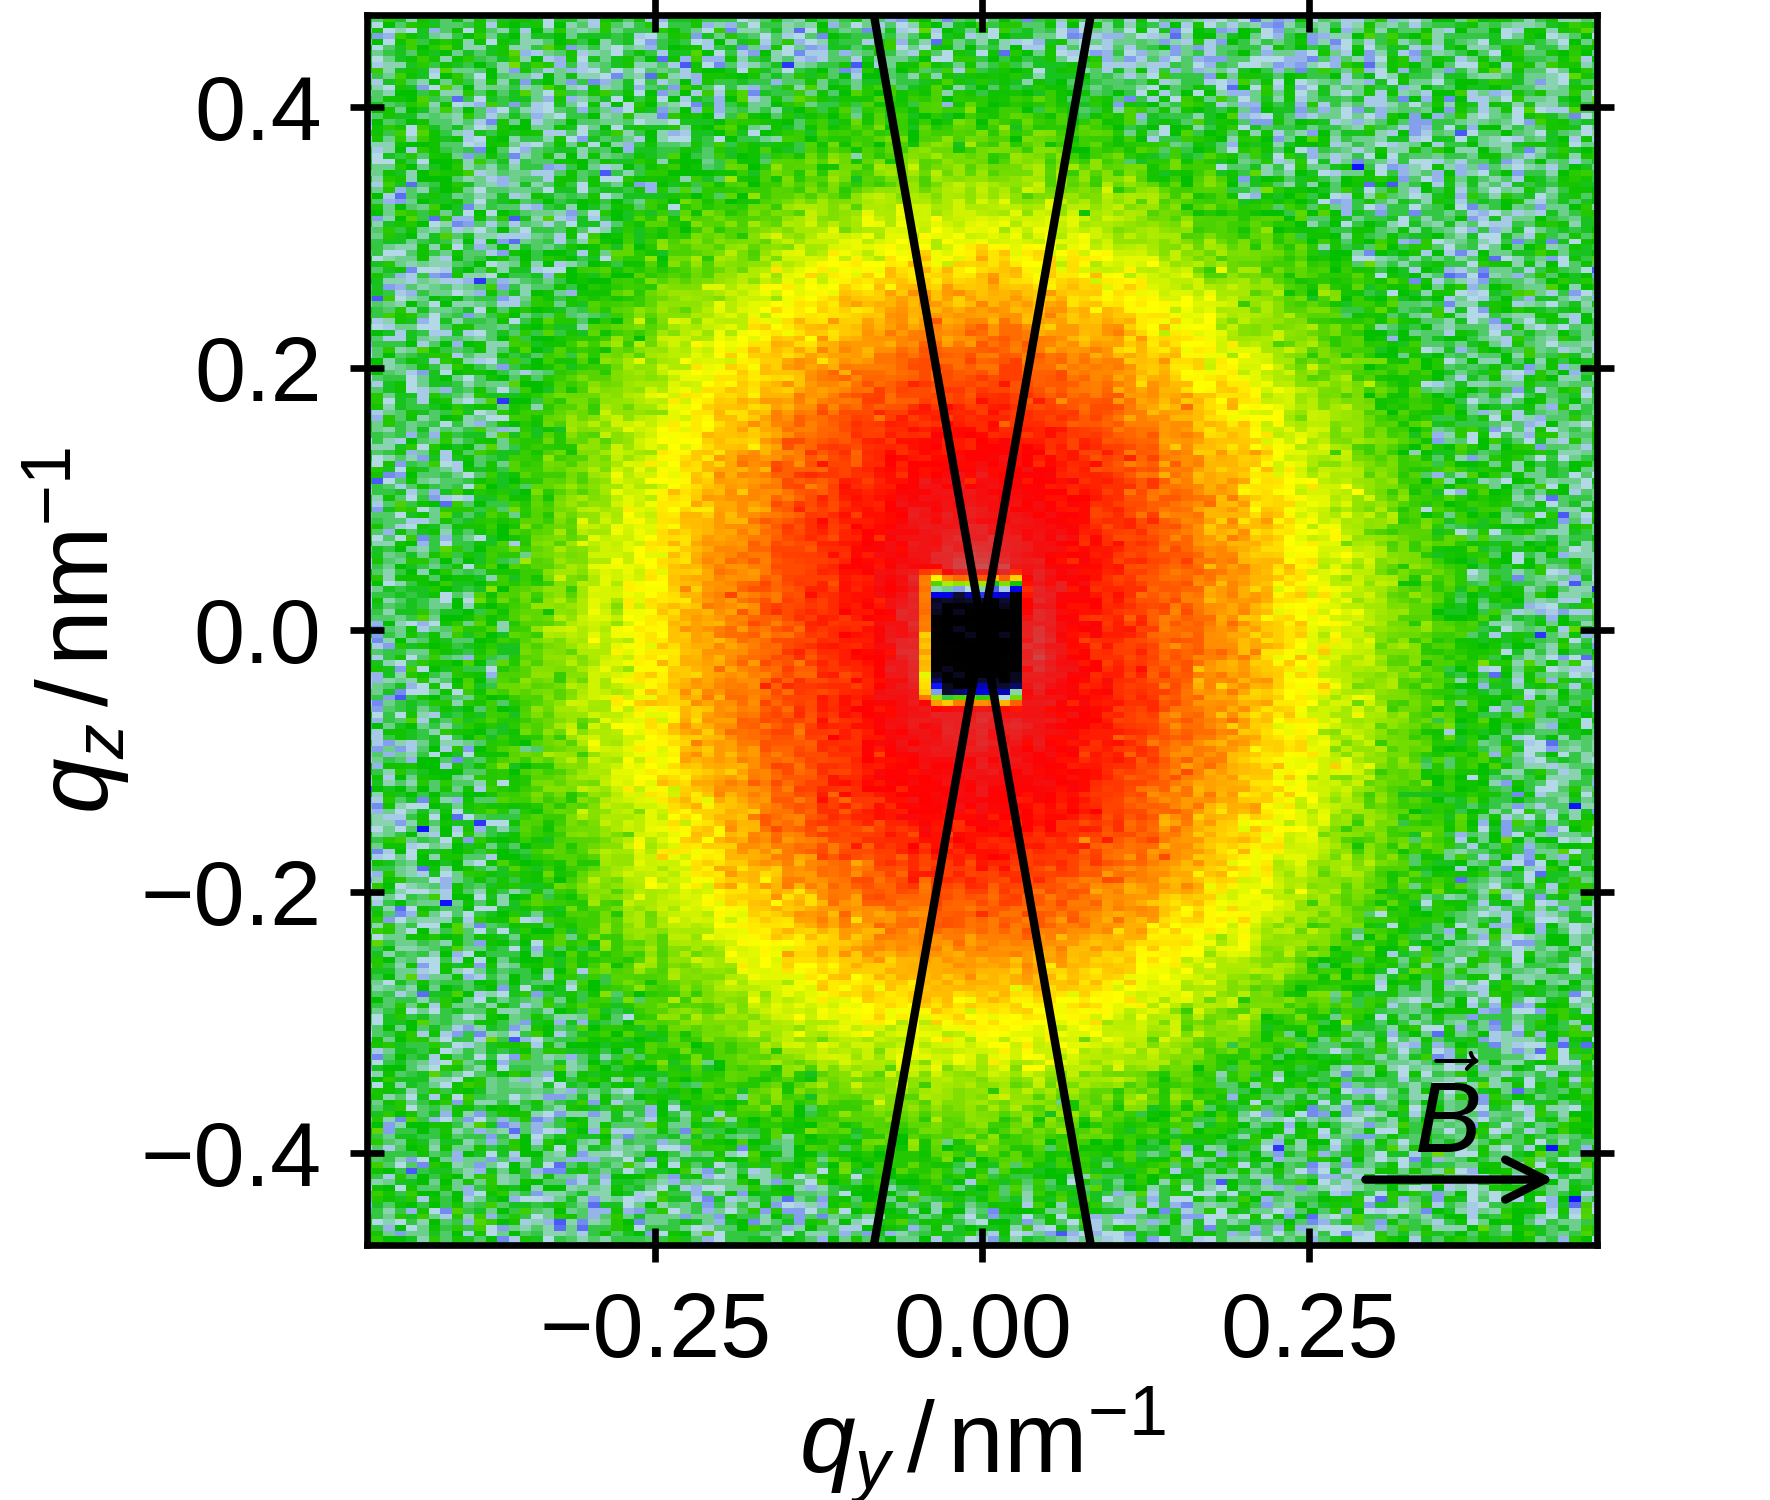
\includegraphics{appendix_methods_SANSPOL_MagneticScattering_RFoff}
      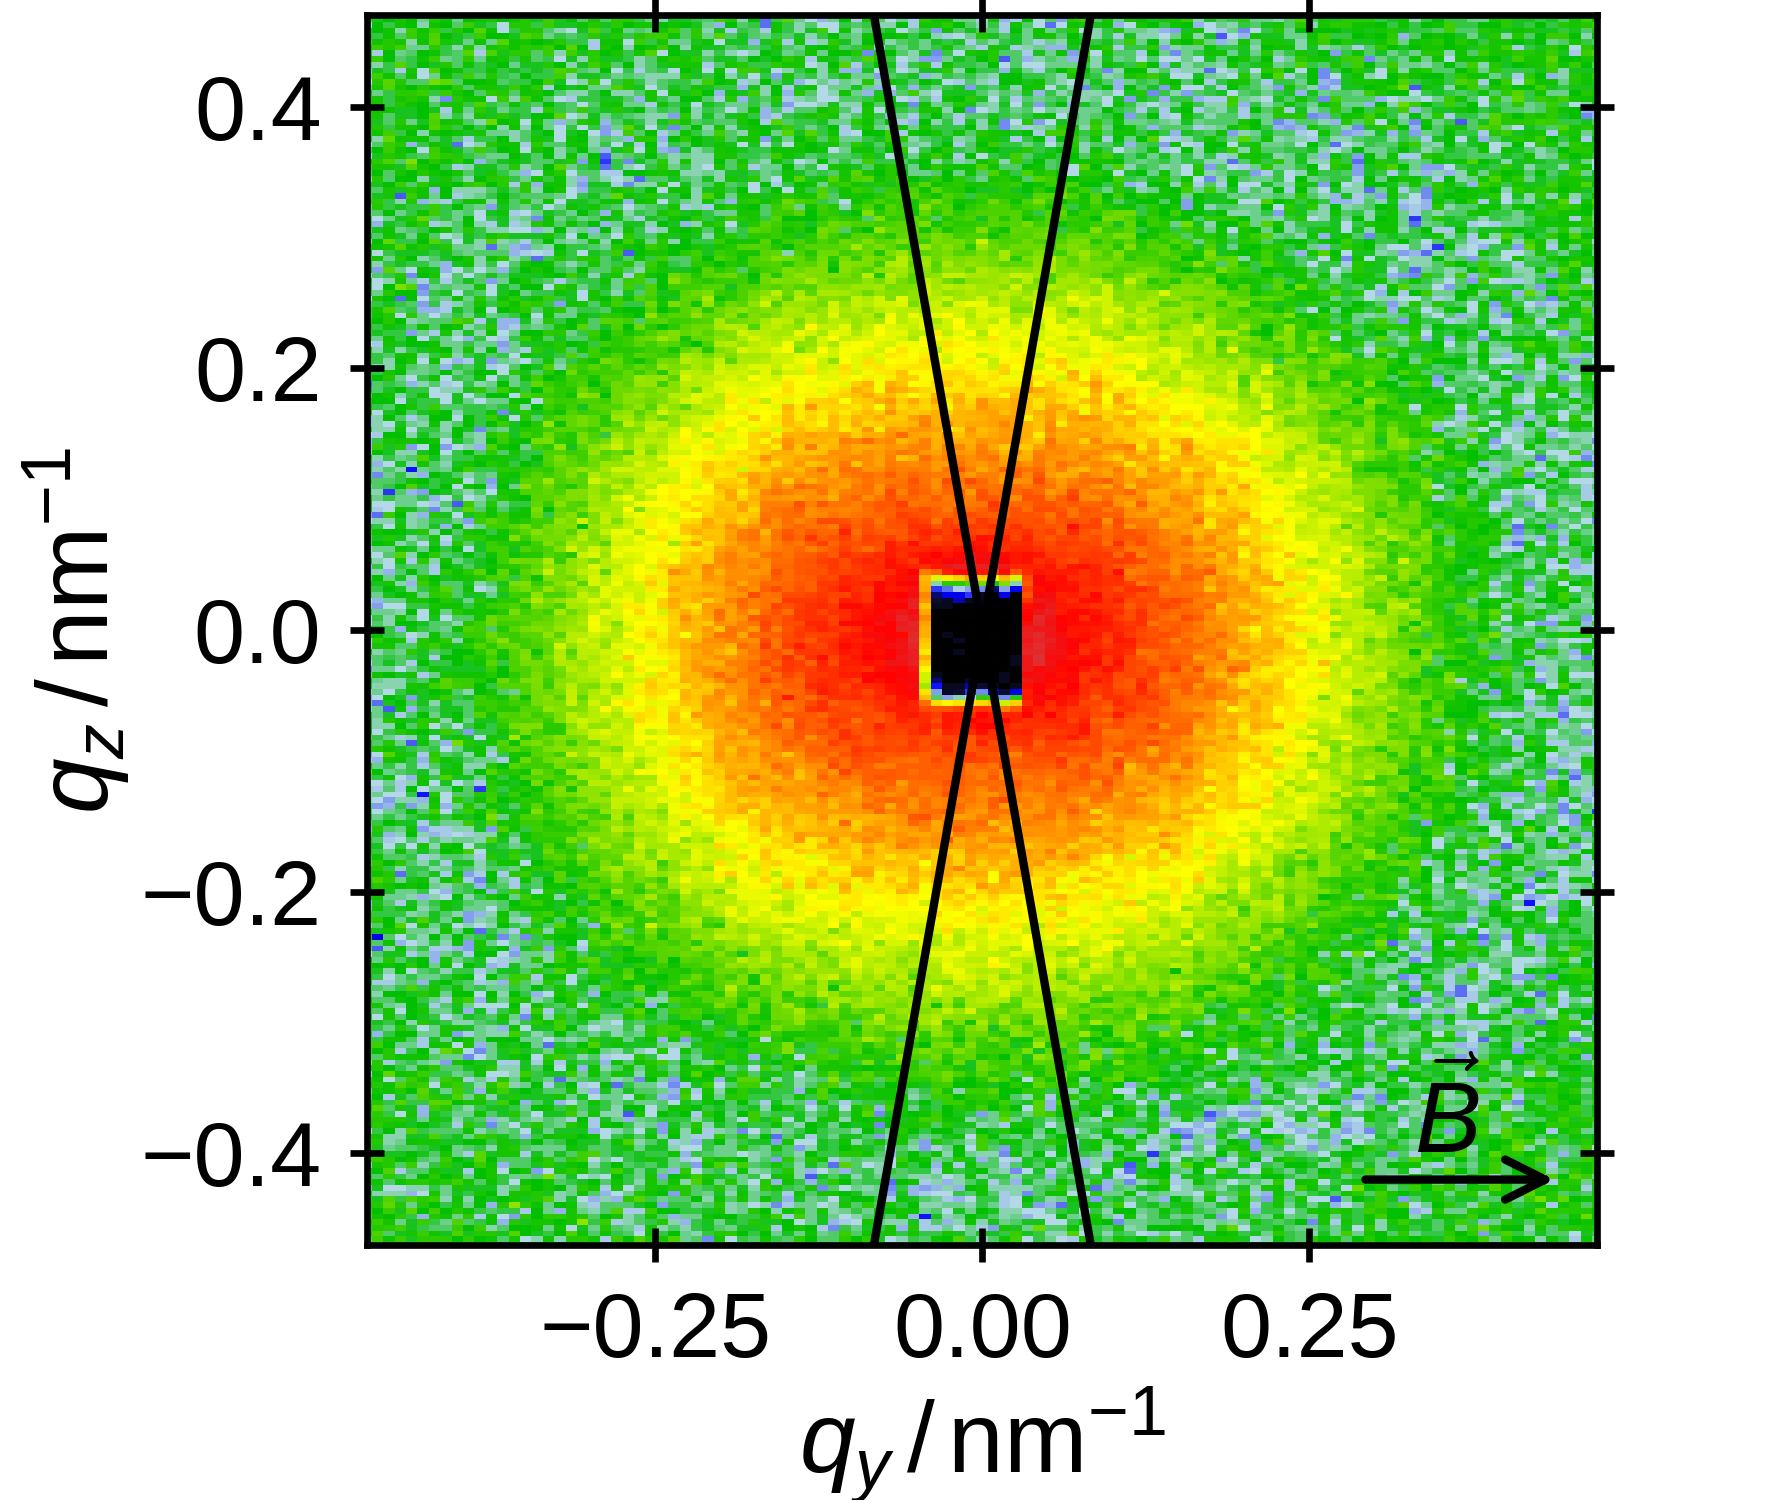
\includegraphics{appendix_methods_SANSPOL_MagneticScattering_RFon}
      \caption{\label{fig:methods:sans:sanspolData}For the evaluation of the magnetic scattering, a cake of $\pm 10^\circ$ is azimuthally integrated along the axis that is perpendicular to the magnetic field (area between black lines).}
    \end{figure}

    When using polarized neutrons in a SANSPOL experiments, two measurements are done for each experiment to obtain the scattering for two neutron spin states.
    Typically, a field to magnetize the sample is applied perpendicular to the beam direction in the lateral plane and parallel to the neutron spin direction.
    As the magnetic scattering only contributes in the plane where the neutron spin is perpendicular to the scattering vector, the scattered intensity pattern on the detector is anisotropic.
    Along the horizontal direction that is parallel to the magnetic field and the neutron spin, only pure nuclear scattering is measured, whereas on the horizontal direction the sum of both nuclear and magnetic scattering contributes.
    For an arbitrary angle between the scattering vector and the magnetic field $\alpha$, the intensity is thus described by the isotropic intensity from the nuclear form factor amplitude $F_\mathrm{nuc}$ and an anisotropic term that is a combination of both the nuclear and magnetic form factor amplitude $F_\mathrm{mag}$ \cite{Wiedenmann_2001_Small, Kohlbrecher_1997_Magne}
    \begin{align}
        I^+(q)
          &\eq F^2_\mathrm{nuc}(q) + \biggl[ F^2_\mathrm{mag} - 2 P F_\mathrm{nuc}(q) F_\mathrm{mag}(q) \biggr] \sin^2(\alpha),\\
        I^-(q)
          &\eq F^2_\mathrm{nuc}(q) + \biggl[ F^2_\mathrm{mag} + 2 P \epsilon F_\mathrm{nuc}(q) F_\mathrm{mag}(q) \biggr] \sin^2(\alpha).
    \end{align}
    The equation accounts for a non-perfect polarization $P$ and flipping ratio $\epsilon$ in the case of $I^-$.
    The polarization is defined by
    \begin{align}
      P \eq \frac{n^+ - n^-}{n^+ + n^-},
    \end{align}
    with $n^+$ the number of neutrons with spin antiparallel to the field and $n^-$ the number of neutrons parallel to the field.

    In this thesis, typically a small cake slice of $\pm 10^\circ$ around the vertical axis, as depicted in \reffig{fig:methods:sans:sanspolData}, is azimuthally integrated to obtain $I^\pm$.
    In this case, the $\sin^2(\alpha)$ factor evaluates to
    \begin{align}
      \frac{1}{20^\circ} \int_{90^\circ-10^\circ}^{90^\circ+10^\circ} \sin^2(\alpha) \dint \alpha \eq
        \frac{1}{20^\circ} \biggl[ -\frac{1}{4}\sin(2\alpha)+\frac{\alpha}{2} \biggr]_{80^\circ}^{100^\circ} \eq
        0.9899
    \end{align}
    If no cake slicing is performed, the integral evaluates to $0.5$.

    Furthermore, due to the different nature of neutron to X-ray experiments, the instrumental resolution also becomes important in model discussions.
    As the flux of the neutron beam is comparably lower, the thin capillaries from SAXS are replaced by liquid containers with a large area and small thickness, to increase the sample area that is illuminated.
    In this thesis, for all samples flat Hellma quartz cuvettes with a thickness of $1 \unit{mm}$ and an area of approximately  $10x40 \unit{mm^2}$ are used.
    Conversely, a larger illuminated area and beam size in comparison to the previously discussed SAXS experiments, means that due to the larger aperture sizes, the angular divergence is increased and needs to be included in a model.
    Additionally, the pixel size $d_\mathrm{pix}$ of neutron detectors is comparatively larger with $5 \unit{mm}$ and add to the angular uncertainty $\sigma_\theta$, which can be estimated by a combination of both effects.
    The uncertainty in $\sigma_\theta$, as well as the finite spread of the neutron wavelength $\sigma_\lambda$ propagate to an uncertainty in the scattering vector magnitude, which is given for small angles by
    \begin{align}
      \biggl( \frac{\sigma_q}{q} \biggr)^2 \eq \biggl( \frac{\sigma_\theta}{\theta} \biggr)^2 + \biggl(\frac{\sigma_\lambda}{\lambda}\biggr)^2.
    \end{align}

    \begin{figure}[tb]
      \centering
      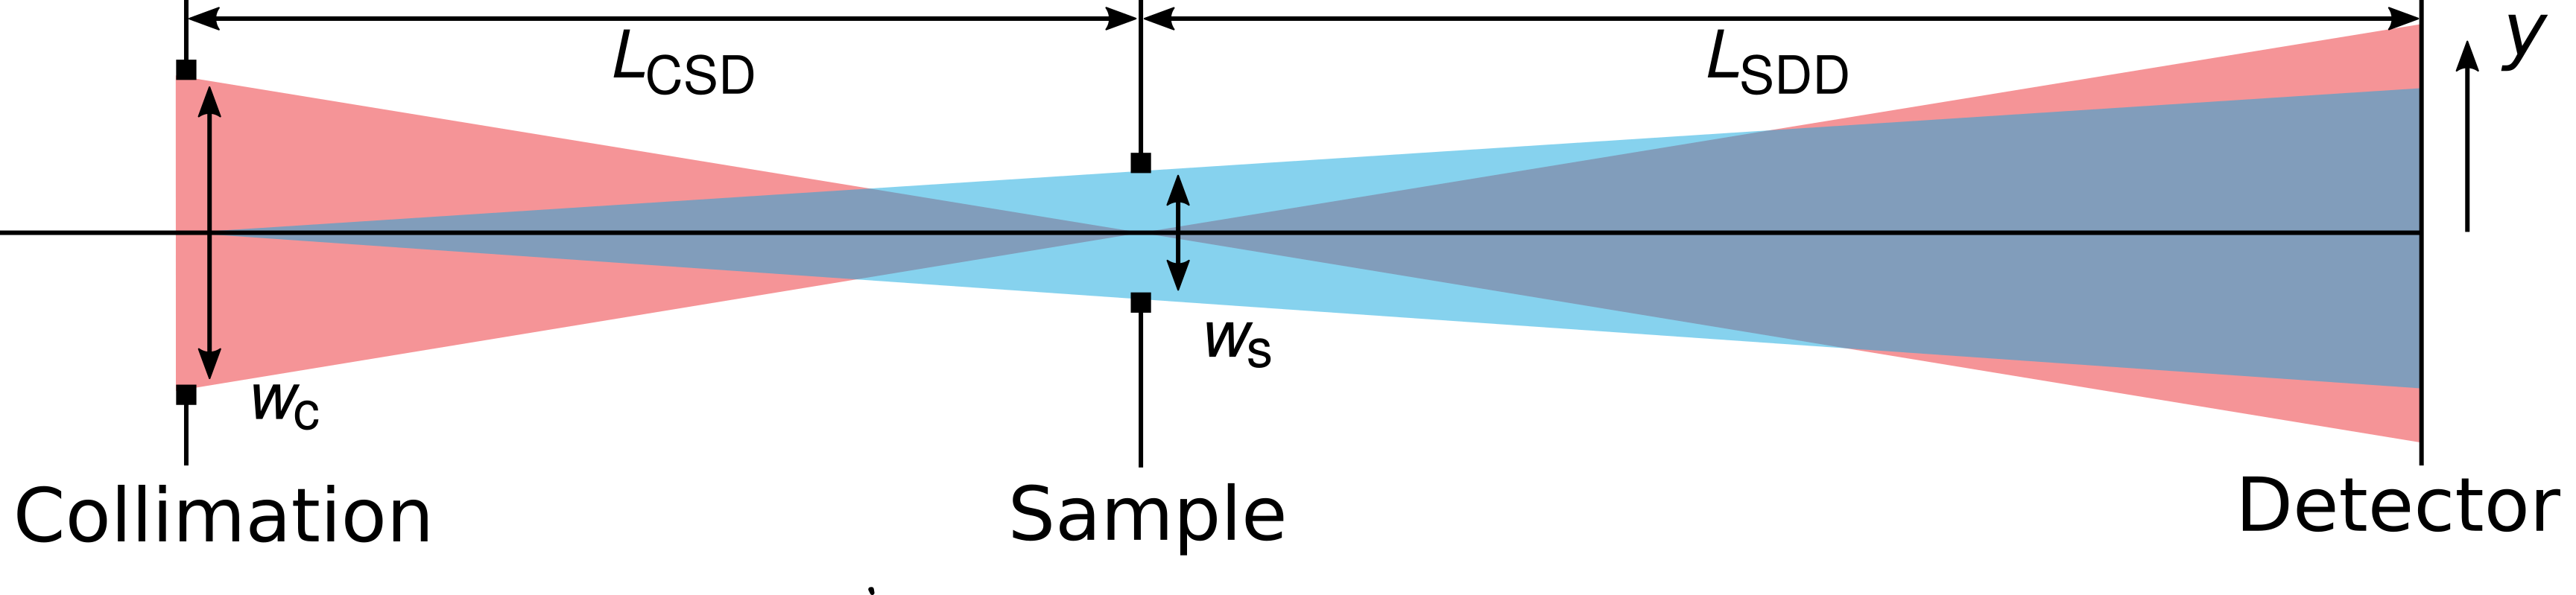
\includegraphics{appendix_methods_sans_resolution}
      \caption{\label{fig:methods:sans:resolution}Depiction of the angular divergence of the direct beam due to finite collimation and sample aperture size.}
    \end{figure}

    The angular divergence due to size of circular apertures is determined by considering the beam spot size on the detector for the direct beam ($q \eq 0$) and assumed to be approximately valid for small-angles as approximation \cite{Pedersen_1990_Analy}.
    The uncertainty in width for the beam spot in a dimension $y$, where the collimation aperture has the width $w_\mathrm{c}$ and the sample aperture the width $w_\mathrm{s}$, is given by \cite{Mildner_2005_Arefr, Hammouda_2006_Thesa}
    \begin{align}
      \sigma_y^2 \eq
        \biggl( \frac{L_\mathrm{SSD}}{L_\mathrm{CSD}} \frac{w_\mathrm{c}}{2} \biggr)^2 +
        \biggl( \frac{L_\mathrm{SSD} + L_\mathrm{CSD}}{L_\mathrm{CSD}} \frac{w_\mathrm{s}}{2} \biggr)^2 +
        \biggl( \frac{d_\mathrm{pix}}{\sqrt{12}} \biggr)^2,
    \end{align}
    with $L_\mathrm{SSD}$ the sample-to-detector distance and $L_\mathrm{CSD}$ the collimation-to-sample distance.
    The first addend can be understood by considering the beam spot due to collimation for $w_\mathrm{s} \eq 0$, as shown in red in \reffig{fig:methods:sans:resolution}, and the second addend by considering conversely $w_\mathrm{c} \eq 0$, as shown in blue.
    The terms assume an equal distribution over the circular apertures and the detector pixel.
    From this, the angular uncertainty is obtained by error propagation
    \begin{align}
      \sigma_{2 \theta} \eq \frac{\sigma_{y}}{L_{\mathrm{SSD}}}.
    \end{align}
    The wavelength spread is typically given for an instrument as the FWHM of the intensity with respect to the wavelength $\Delta \lambda / \lambda$, being typically in the order of $10 \, \%$.
    Assuming a triangular distribution around the mean intensity, the wavelength variance is determined by
    \begin{align}
      \biggl( \frac{\sigma_\lambda}{\lambda} \biggr)^2 \eq \frac{1}{6} \biggl( \frac{\Delta \lambda}{\lambda} \biggr)^2.
    \end{align}
    The prefactor is determined by the shape of the wavelength distribution. For an equidistributed shape, it would be $1/12$ and for a Gaussian distribution $1/\sqrt{8\log(2)}$.

    Combining all effects into a single equation for the variance of the scattering vector, it can be estimated by
    \begin{align}
      \begin{split}\label{eq:methods:sans:instrumentalResolution}
        \sigma_q^2
        &\eq
          \biggl( \frac{2\pi}{\lambda} \biggr)^2 \biggl[ \biggl( \frac{w_\mathrm{c}}{2 L_\mathrm{CSD}} \biggr)^2 +
          \biggl( \frac{L_\mathrm{SSD} + L_\mathrm{CSD}}{L_\mathrm{CSD}} \frac{w_\mathrm{s}}{2 L_\mathrm{SSD}} \biggr)^2 +
          \biggl( \frac{d_\mathrm{pix}}{\sqrt{12} L_\mathrm{SSD}} \biggr)^2 \biggr] \\
        &\hspace{1cm}+ \frac{1}{6} \biggl( \frac{\Delta \lambda}{\lambda} \biggr)^2 q^2 .
      \end{split}
    \end{align}
    This gives a good estimate for the order of magnitude of the resolution.
    In real experiments there are however additional effects, from the instrumental setup, gravity \etc, which are not included.
    Therefore it is chosen in this thesis, to keep $\sigma_\theta$ as a adjustable parameter, and only to use the formula to confirm that the value is in the expected order of magnitude.

    The instrumental resolution is included in a model by smearing the calculated intensity for a form factor with a Gaussian function via
    \begin{align}
      I_\mathrm{smeared} (q) \eq \frac{1}{\sqrt{2 \pi}\sigma_q}  \int I(q^\prime) \exp\biggl(-\frac{(q - q^\prime)^2}{2 \sigma_q^2}\biggr)\dint q^\prime
    \end{align}
    As the resolution depends on the sample-to-detector distance and collimation distance, measurements taken at a short and long detector distance are not merged to one single data set for evaluation.
    Instead they are treated separately, where each model is smeared by its respective angular divergence parameter $\sigma_\theta$, but otherwise sharing the remaining model parameters.
\end{document}